\documentclass[a4j,12pt,onecolumn,oneside,final]{jreport}

%\usepackage{gthesis}
\usepackage{gthesis_myown}

\usepackage{amsmath,amsthm,amssymb,ascmac}
\usepackage{fancybox}
\usepackage{slashbox}
%\usepackage[dviout]{color,graphics}
%\usepackage{graphicx}
\usepackage[dvipdfmx]{graphicx}
%\usepackage{color}
\usepackage[dvipdfmx]{color}
\usepackage{psfrag}
%\usepackage{upgreek}
\usepackage{bm}
\usepackage{wrapfig}
\usepackage{algorithmic,algorithm}
\usepackage{subcaption}
%%%%%%%%%%%%%%%%%%%%%%%%%%%%%%%%%%%%%%%%%%%%%%%%%%%%%%%%%%%%%%%%
% put local tex-macros in this file %

%%%%%%%%%%%%%%%%%%%%%%%%%%%%%
%色設定
%%%%%%%%%%%%%%%%%%%%%%%%%%%%%
\definecolor{Black}{rgb}{0.0,0.0,0.0}
\definecolor{Red}{rgb}{0.9,0.0,0.1}
\definecolor{Blue}{rgb}{0.1,0.1,0.5}
\definecolor{Green}{rgb}{0.1,0.4,0.1}
\definecolor{Gray}{rgb}{0.75,0.85,0.9} % Fuji-iro
\definecolor{Shade}{rgb}{0.1,0.1,0.4}

%%%%%%%%%%%%%%%%%%%%%%%%%%%%%%%%%%%%%%%%%%%%%%%%%%%%%%%%%%%%%%%%
\年度{平成27年度}
%\提出年月{平成27年7月}
\提出年月{平成28年2月}

\題名{一つ以上の参照点を考慮した\\物体移動動作の学習と再現に関する研究}
\梗概題名{一つ以上の参照点を考慮した\\物体移動動作の学習と再現に関する研究}
\指導教員名A{長谷川 修}
\職名A{准教授}

\指導教員名B{}
\職名B{}

%\所属学科{電気電子工学科}{}
\所属学科{情報工学科}{}
\学籍番号{12\_06181}
\氏名{菰田 徹也}

\内容梗概{人間の生活環境で活動する汎用ロボットの実現には,人間とのインタラクションを通じて動作を学習する能力が望ましく,その実現を目指した研究として模倣学習が存在する.しかし,模倣学習
の研究で扱われているものの多くの先行研究では,教示動作の目標位置即ちその動作が目標とする最終状態について教示者とロボット間で既知で共有されているという前提に立っている.そこで本研究では,環境中の一つ以上の参照点に応じて目標位置が決定されるような物体移動動作を教示し,その動作がどの参照点に対してどのように決定されるかを表す観点を推定し,再現する手法を提案する.

初めに,環境中の参照点に対応した観点それぞれに学習モデルとしてガウスモデルを生成する.この際環境中の各物体の位置を参照点に含めると同時に任意の物体間の重心位置も参照点として考慮することで複数の物体の位置関係を考慮した動作の学習を可能にしている.
学習時には教示された物体移動動作を各参照点を原点とした相対位置に変換し,観点に応じた線形変換を行ったうえで各確率モデルを更新する.
再現時には学習された確率モデルのうち,最もばらつきの小さい観点を教示者が意図していた観点だと推定してベクトルを生成し,観点に応じた逆線形変換を行ったうえで参照点の座標を加えて動作の目標位置を推定する.

また,学習した確率モデルからの生起確率を用いることで,例示動作が既学習動作のいずれであるかを識別することも可能になる.

有効性を検証するため,提案手法を用いて学習させた動作を学習時と異なる初期環境で再現,識別させる実験を行った.結果として,複数の参照点間の相対位置を考慮した動作を学習できていることが示された.

今後の課題としては,複数の段階を持つより高度な動作の学習手法や,目標位置や被動作物体の決定時に位置情報以外の特徴量を考慮できるより一般的な学習手法の考察が挙げられる.}


\begin{document}
% ----------------------------------------------------------------------
% 表紙
\maketitle
% ----------------------------------------------------------------------
% 目次
\setcounter{page}{1}
\renewcommand{\thepage}{\roman{page}}
\setcounter{tocdepth}{1}
\tableofcontents
\clearpage
% ----------------------------------------------------------------------
% 内容
\setcounter{page}{1}
\renewcommand{\thepage}{\arabic{page}}
%\chapter{Introduction}
\chapter{序論}

\section{背景}

近年のロボット技術の発展により,人間の生活環境で活躍する汎用ロボットの実現に向けた様々な研究が行われている.汎用ロボットとは,工場などで作業を行うようなあらかじめプログラムされた動作を繰り返すものではなく,環境との相互作用によって適切な行動を学習,選択して実行できる能力を持ったロボットのことである.人間の生活環境で活躍する汎用ロボットには,人間とのインタラクションを通じて動作の方法や内容を学習する能力が必要不可欠である.
人間とのインタラクションを通じて学習を行う手法の研究として,人間の教示動作を観測しそれを模倣することによって,ロボットがその動作を再現するにはどのようにすればいいかを学習する模倣学習があるが,人間の動作を模倣するだけではその動作を理解したとは言えない.
例えばロボットに,コップを運ぶという動作を教示して再現させることを考える.ある時点で食器棚に置かれているコップを,その時点でテーブルの一角に座る人の前に動かす動作を見せた場合,単純に教示動作からコップの最終位置を把握したとしても,それはそのテーブルの一角という場所に動かすことが重要なのか,その座っている人の前に動かすことが重要なのかが理解できていなければ,人の座る位置やテーブルの位置などの環境が変わった場合に教示者の意図に正しく沿った動作が再現できない.このような問題を解決するためには,特定の初期状態から人間がどのように動作したかという明示的な情報から,人間がその動作を行う際に環境中のどの情報を意識しているかという暗黙的な情報を推測し,動作における観点を人間とロボット間で共有する必要がある.
このような背景から,本研究では教示者の動作から動作意図を把握し,意図を汲み取った動作を再現できるようなロボットの実現に向けた研究として,一つ以上の参照点との相対位置に応じて目標位置が決定する物体移動動作の教示から,教示者の着目している参照点とそれに対する位置決定の方法を推定する手法を提案する.

\section{関連研究について}

人間とロボットのインタラクションの分野において,
人間の教示動作によるロボットの模倣学習に関する様々な研究が行われている.(\cite{imitation1}-\cite{imitation4})模倣学習とはロボットに対し,タスクや動作をあらかじめプログラムするのではなく,ロボットの腕を直接操作したり,人間の動作を視覚的に与えるなどで動作を教示し,その挙動を模倣することでタスクや動作を学習する手法を研究する分野である.その際に教示者とロボット間のキネマティクスなどの制約の違いを克服する機構を持たせることで,ロボットへの動作教示をより自然,適切に行う手法に関する研究が行われている.
中岡\cite{nakaoka}は,教示した人の舞踊動作から四肢の長さや関節角などを考慮した見真似学習を行い,同時に安定した姿勢を保ち直立を維持した状態でロボットに舞踊動作を模倣させる研究を行った.このようにロボットに対し,教示動作と類似した動作を再現させる手法としての模倣学習は成功している.一方,特定のタスクを達成させることを目的とした模倣学習も数多く研究されている.
Schaal\cite{schaal}は,バネマスダンパで構成される運動モデルのパラメータを教示動作から学習することで,ドラムをたたくなどの周期運動や,ラケットでボールを打つなどの到達運動の再現を行っている.このように,目標位置が既知で教示者とロボットの間で共通に認識されているという前提で,その目標位置までどのように動作するかを扱う研究は多く存在するが,動作教示の煩わしさを軽減し,人とロボットのインタラクションを円滑にするためには,動作の目標位置などの教示者の内包する意図は明示的に与えるより,教示動作からロボットが推測し,教示者は教示動作を見せるだけでよくなることが望ましい.そのため,目標位置はロボット自身が教示動作から推定する機構を持たなければならないが,目標位置の決定方法は動作によって異なる.例えば物体移動動作において,ある物体を右に動かすという動作はその物体の位置が最終位置の決定にかかわるが,一方の物体を他方の物体に近づけるという動作は2つの物体間の位置関係が最終位置の決定に必要になる.これには,目標位置決定の基準となる参照点と,その参照点に対してどのような位置,状態かを表す変位の2つを推定する必要がある.
杉浦ら\cite{sugiura}は動詞の持つ動作概念を人とロボット間で共有することを目標にした研究を行った.その中で物体移動動作の教示に関して,各オブジェクトの位置を参照点とし,複数の座標系に変換した動作軌跡を生成する隠れマルコフモデルを学習して最尤推定によって参照点と変位を決定し,参照点を考慮した動作概念の獲得を行った.またDongら\cite{dong}は,動作と参照点の関係である変位を,参照点に到達する,参照点から出発する,位置遷移量が等しい,などの特徴的な数パターンに大別し,動作軌跡を生成している.これらの研究はいずれも,動作の概念として参照点に対する動作軌跡を獲得することを目標としており,参照点の決定方法及び選択肢に関しては簡単な議論にとどまっている.
そのため,これらの手法では動作の目標位置の学習に十分とは言えず,表現できない動作が存在する.特にこれら従来手法では学習できない動作として,複数の参照点間の位置関係を考慮した動作が挙げられる.例えば椅子を等間隔に並べるという動作を考えた時,椅子1つ1つを参照点として考えても,椅子の位置関係が2つ以上の椅子の位置で決定し,かつ毎回変化しうるものであるため適切に学習することができない.このような動作を適切に学習するためには,2つ以上の物体の位置を考慮した参照点の決定方法が備わっていなければならない.本研究では,これら関連研究で用いられる手法を参考にしつつ,特に複数の物体を参照点として考慮する必要のある動作の学習を目標として,より多種の動作意図を取得する方法を提案する.        

\section{本論文の構成}


%\chapter{Numerical Examples}
\chapter{従来手法}

\section{問題設定と定義}

本研究は静的な環境下で教示される物体移動動作から,被移動物体(以下,トラジェクタ)の目標位置の決定に関与する参照点と変位を推定する手法について提案する.
そのため本研究では,ある地点に置いてある物体を参照点と変位に従った他の地点に移動するという,初期状態と最終状態の対を動作と定義する.

本文において,参照点を$l$,変位を$k$と表し,参照点と変位の対$<l , k>$を観点と定義する.また$L , K , V$をそれぞれ参照点の候補の集合,変位の候補の集合,観点の候補の集合とする.
従って本研究の主たる目的は,与えられた教示動作から観点$<l , k>$を推定し,観点に従った動作を再現することである.

\section{従来手法の概要}

\subsection{参照点}

杉浦ら\cite{sugiura}の手法において,参照点は環境中の物体の位置,トラジェクタの初期位置(動作開始点),画面中央と設定されている.
トラジェクタの遷移には,大別すると以下の3種類が存在するとしている.

	\begin{enumerate}
		\item 初期状態に関わらず,トラジェクタの初期位置に対して一定の遷移を行う
		\item 初期状態に関わらず,空間上の特定の位置に遷移を行う
		\item 他の物体との相対位置に応じて遷移先が変化する
	\end{enumerate}
これら3種類の違いについてFig.\ref{figure:2_moving_trajector}で示す.

%%%%%%%%%%%%%%%%%%%%%%%%%%%%%%%%%%%%%%%%%%%%%%%%%%%%%%%%%%%%%%%%%%%%%%%%%%%%%%%%%%%%%%%%%%%%%%%%%%%%%%%
\begin{figure}[h]
	\centering
	\begin{minipage}[t]{.3\textwidth}
		\centering
		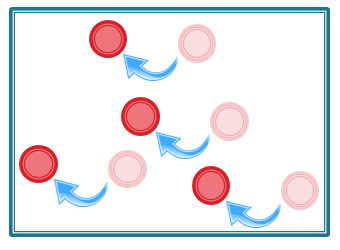
\includegraphics[width=4.7cm]{figure1_sub_a.png} \\ %TeXの基本として, \\ で緊急改行ができる.(今回の場合や行列などを除き,あまり使わない)
		\subcaption{トラジェクタ初期位置に対して一定}
		\label{subfigure:2_moving_trajector1}    
	\end{minipage}
	\begin{minipage}[t]{.3\textwidth}
		\centering
		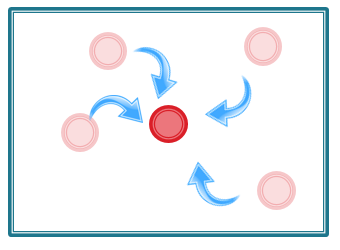
\includegraphics[width=4.7cm]{figure1_sub_b.png} \\ %TeXの基本として, \\ で緊急改行ができる.(今回の場合や行列などを除き,あまり使わない)
		\subcaption{空間上の特定の位置}
		\label{subfigure:2_moving_trajector2}
	\end{minipage}
	\begin{minipage}[t]{.3\textwidth}
		\centering
		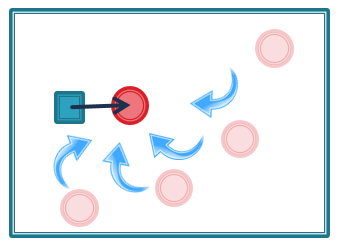
\includegraphics[width=4.7cm]{figure1_sub_c.png} \\ %TeXの基本として, \\ で緊急改行ができる.(今回の場合や行列などを除き,あまり使わない)
		\subcaption{他物体の位置に応じて変化}
		\label{subfigure:2_moving_trajector3}
	\end{minipage}
	\caption{トラジェクタ遷移の違い}
	\label{figure:2_moving_trajector}
\end{figure}
%%%%%%%%%%%%%%%%%%%%%%%%%%%%%%%%%%%%%%%%%%%%%%%%%%%%%%%%%%%%%%%%%%%%%%%%%%%%%%%%%%%%%%%%%%%%%%%%%%%%%%%
Fig.\ref{subfigure:2_moving_trajector1}はトラジェクタの初期位置を,Fig.\ref{subfigure:2_moving_trajector2}は画面中央を参照点に含めることで,Fig.\ref{subfigure:2_moving_trajector3}の特殊な事例として実現できるため,全ての物体移動動作は参照点との相対位置を考慮した目標位置を持つとしている.

このような理由から,従来研究では$L$を各物体の位置,トラジェクタの動作開始点,画面中央に定めている.

\subsection{変位}

特定の参照点に対し,変位の違いによって動作はさらに以下の2種類が存在すると定義されている.

	\begin{enumerate}
		\item 参照点を原点とし,常に一定の相対位置に遷移する
		\item 参照点を原点とし,トラジェクタの初期位置に応じて遷移先が変化する
	\end{enumerate}
これら2種類の違いについてFig.\ref{figure:2_difference_displacement}で示す.
%%%%%%%%%%%%%%%%%%%%%%%%%%%%%%%%%%%%%%%%%%%%%%%%%%%%%%%%%%%%%%%%%%%%%%%%%%%%%%%%%%%%%%%%%%%%%%%%%%%%%%%
\begin{figure}[h]
	\centering
	\begin{minipage}[t]{.4\textwidth}
		\centering
		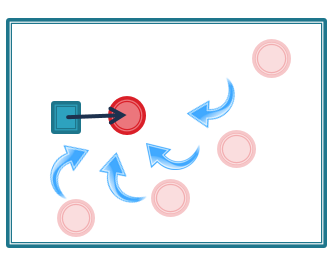
\includegraphics[width=6cm]{figure2_2_sub_a.png} \\ %TeXの基本として, \\ で緊急改行ができる.(今回の場合や行列などを除き,あまり使わない)
		\subcaption{一定の相対位置}
		\label{subfigure:2_difference_displacement1}    
	\end{minipage}
	\begin{minipage}[t]{.4\textwidth}
		\centering
		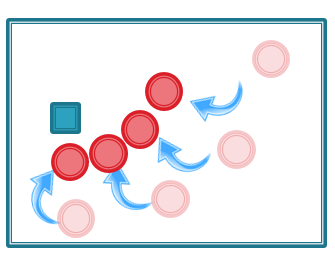
\includegraphics[width=6cm]{figure2_2_sub_b.png} \\ %TeXの基本として, \\ で緊急改行ができる.(今回の場合や行列などを除き,あまり使わない)
		\subcaption{トラジェクタの初期位置に応じて変化}
		\label{subfigure:2_difference_displacement2}
	\end{minipage}
	\caption{参照点に対する遷移の違い}
	\label{figure:2_difference_displacement}
\end{figure}
%%%%%%%%%%%%%%%%%%%%%%%%%%%%%%%%%%%%%%%%%%%%%%%%%%%%%%%%%%%%%%%%%%%%%%%%%%%%%%%%%%%%%%%%%%%%%%%%%%%%%%%
Fig.\ref{subfigure:2_difference_displacement1}は例えばトラジェクタを物体の右隣に動かすという動作などで,参照点である物体に関して常に相対位置が一定である.Fig.\ref{subfigure:2_difference_displacement2}はトラジェクタを物体に近づけるという動作などで,これは参照点となる物体とトラジェクタの初期位置の位置関係によって,参照点からの目標位置の相対位置が変化する.

従来手法ではこれらを判別する変位$k$としてそれぞれに異なる座標系を対応させている.例えばFig.\ref{subfigure:2_difference_displacement1}の動作では,参照点を原点として画面に平行な座標系を考慮することで実現することができ,Fig.\ref{subfigure:2_difference_displacement2}の動作では,参照点を原点としてトラジェクタの動作開始点に軸を向けた座標系を考慮することで実現することができる.

以下,本研究では変位$k$は座標系によって表されるとし,$Fig.\ref{subfigure:2_difference_displacement1}$のような画面空間に平行な座標系を恒等座標$k_{id}$,Fig.\ref{subfigure:2_difference_displacement2}のような,トラジェクタの動作開始点に向けた軸を持った座標系をランドマーク-トラジェクタ座標$k_{lt}$と定義する.

\subsection{学習,再現}

従来手法では教示動作が与えられたとき,以下の式を用いて尤度が最大となる参照点$\hat{l}$,座標系$\hat{k}$,隠れマルコフモデルのパラメータ$\hat{λ}$を最尤推定により学習している.
\begin{equation}
	\label{equation:sugiura}
	(\hat{λ} , \hat{k} , \hat{l}) = \mathop{\arg\max}_{λ , k , l}\sum_{i=1}^{N}\log P(F(Y_{i} , k , l_{i}) ; λ)
\end{equation}
ここで,$Y_{i}$はトラジェクタの位置,速度,加速度の時系列データ,$l_{i}$は参照点,$F(Y , k , l)$は座標系$k$,参照点$l$としたときのトラジェクタの動作軌道,$P(F,λ)$は動作軌道$F$がパラメータ$λ$の確率モデルから生成される確率である.杉浦らの研究では動作軌道を再現することを目標の一つとしていたため,確率モデルに時系列データを扱える隠れマルコフモデルを使用している.動作再現は\ref{equation:sugiura}式の最尤推定によって推定されたパラメータ$λ$を持つ隠れマルコフモデルからトラジェクタ遷移情報の時系列を生成することで実現する.

%\chapter{Preliminaries}



\chapter{提案手法}

そのような問題点を踏まえ、提案手法では複数の参照点を学習に利用する手法を導入した。従来手法の拡張で複数の参照点を考慮できるようにするためには、参照点と変位(座標系)のいずれかに複数の参照点の情報を保持する機構を導入する必要がある。そこで参照点の候補に各参照点間の重心位置を採用することによって、参照点に複数の参照点の位置情報を含めることができると考えた。また本研究では物体移動動作を初期状態に対する最終状態の決定と定義し、動作中のトラジェクタ軌跡に関しては考えていないため、学習モデルはより単純なガウスモデルを使用した。
重心位置を参照点として考慮した際、構成する参照点同士の位置関係に対応した相対位置を学習するために、重心位置を原点として重心を構成する参照点の向きに軸を取る座標系を考慮する必要がある。そのため、重心位置に対する変位にはその構成参照点の数分の座標系を追加生成する。

\subsection{参照点}

従来手法で採用されていた各物体位置、トラジェクタの初期位置、画面中央に加えて、提案手法では新たに2つ以上の任意の物体間の重心位置を参照点に含めた。即ち環境中の$n$個の物体に対して、参照点は$2^{n}$個考慮する。

\subsection{変位}

従来手法で考慮されていた2つの変位に加えて、複数の物体を考慮した動作の学習を実現するために提案手法では以下の3種類が存在するとした。

	\begin{enumerate}
		\item 参照点を原点とし、常に一定の相対位置に遷移する
		\item 参照点を原点とし、トラジェクタの初期位置に応じて遷移先が変化する
		\item 複数の物体の位置関係に応じて遷移先が変化する
	\end{enumerate}
これら3種類の違いについてFig.\ref{figure:difference_displacement}で示す。
%%%%%%%%%%%%%%%%%%%%%%%%%%%%%%%%%%%%%%%%%%%%%%%%%%%%%%%%%%%%%%%%%%%%%%%%%%%%%%%%%%%%%%%%%%%%%%%%%%%%%%%
	\begin{figure}[t]
%中央ぞろえ
		\begin{center}
			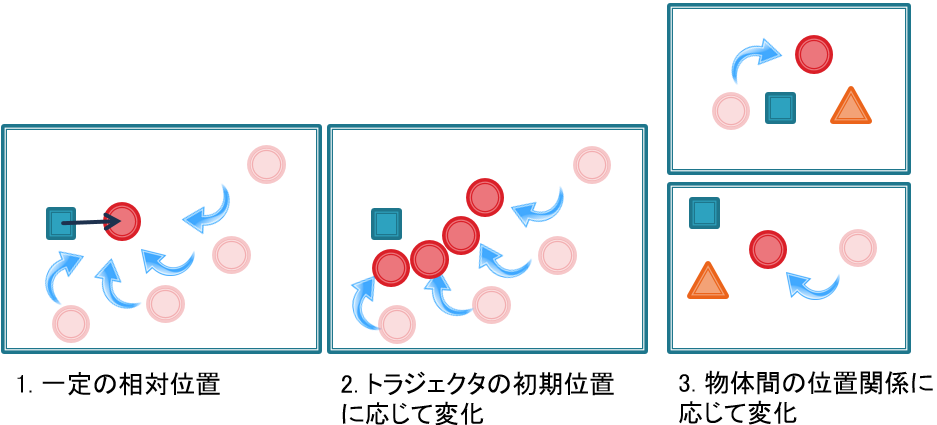
\includegraphics[width=14cm]{figure2.png} \\ %Teの基本として, \\ で緊急改行ができる。(今回の場合や行列などを除き、あまり使わない)
			\caption{参照点に対する遷移の違い}
			\label{figure:difference_displacement}
		\end{center}
	\end{figure}
%%%%%%%%%%%%%%%%%%%%%%%%%%%%%%%%%%%%%%%%%%%%%%%%%%%%%%%%%%%%%%%%%%%%%%%%%%%%%%%%%%%%%%%%%%%%%%%%%%%%%%%

3の例として、トラジェクタをある物体とある物体の間に動かすという動作などがあり、これは複数の物体を考慮した参照点の設定を行う必要がある。

\section{動作学習}

与えられた教示動作から、各観点のガウスモデルを学習する。まず教示動作の目標位置の、各参照点を原点とした相対位置を求め、各座標系ごとに座標変換、正規化を行う。それにより得たベクトル$v$を用いて、各ガウスモデルの平均$μ$、2乗平均$Q$、分散$σ$を以下のように更新する。

\[
	μ  \leftarrow \frac{N}{N+1}μ+\frac{1}{N+1}v
\]
\[
	Q  \leftarrow \frac{N}{N+1}Q+\frac{1}{N+1}v^2	
\]
\[
	σ  \leftarrow Q - μ^2
\]

動作学習のアルゴリズムの詳細については付録\ref{appendix3}に示す。


\section{動作再現}

教示動作から学習された各観点における確率モデルを用いて、異なる初期環境での動作再現を行う。まず学習された各観点のガウスモデルのうち最も分散の小さいものを探索する。分散が小さいとは教示動作がその観点に対して常に類似した目標位置に遷移していたということであり、教示者が意図していた参照点と変位である可能性が高いと考えられる。探索された分散の最小である観点のガウスモデルの平均を、その観点と再現時の初期環境に応じた正規化と座標変換の逆関数を計算し、初期環境における参照点の位置に平行移動することで再現動作のトラジェクタの目標位置を推定する。
Fig.\ref{figure:learning_and_reproduction_model}に、提案手法における動作学習と動作再現の模式図を示す。
また付録\ref{appendix3}に、動作再現のアルゴリズムの詳細を示す。
%%%%%%%%%%%%%%%%%%%%%%%%%%%%%%%%%%%%%%%%%%%%%%%%%%%%%%%%%%%%%%%%%%%%%%%%%%%%%%%%%%%%%%%%%%%%%%%%%%%%%%%
	\begin{figure}[h]
%中央ぞろえ
		\begin{center}
			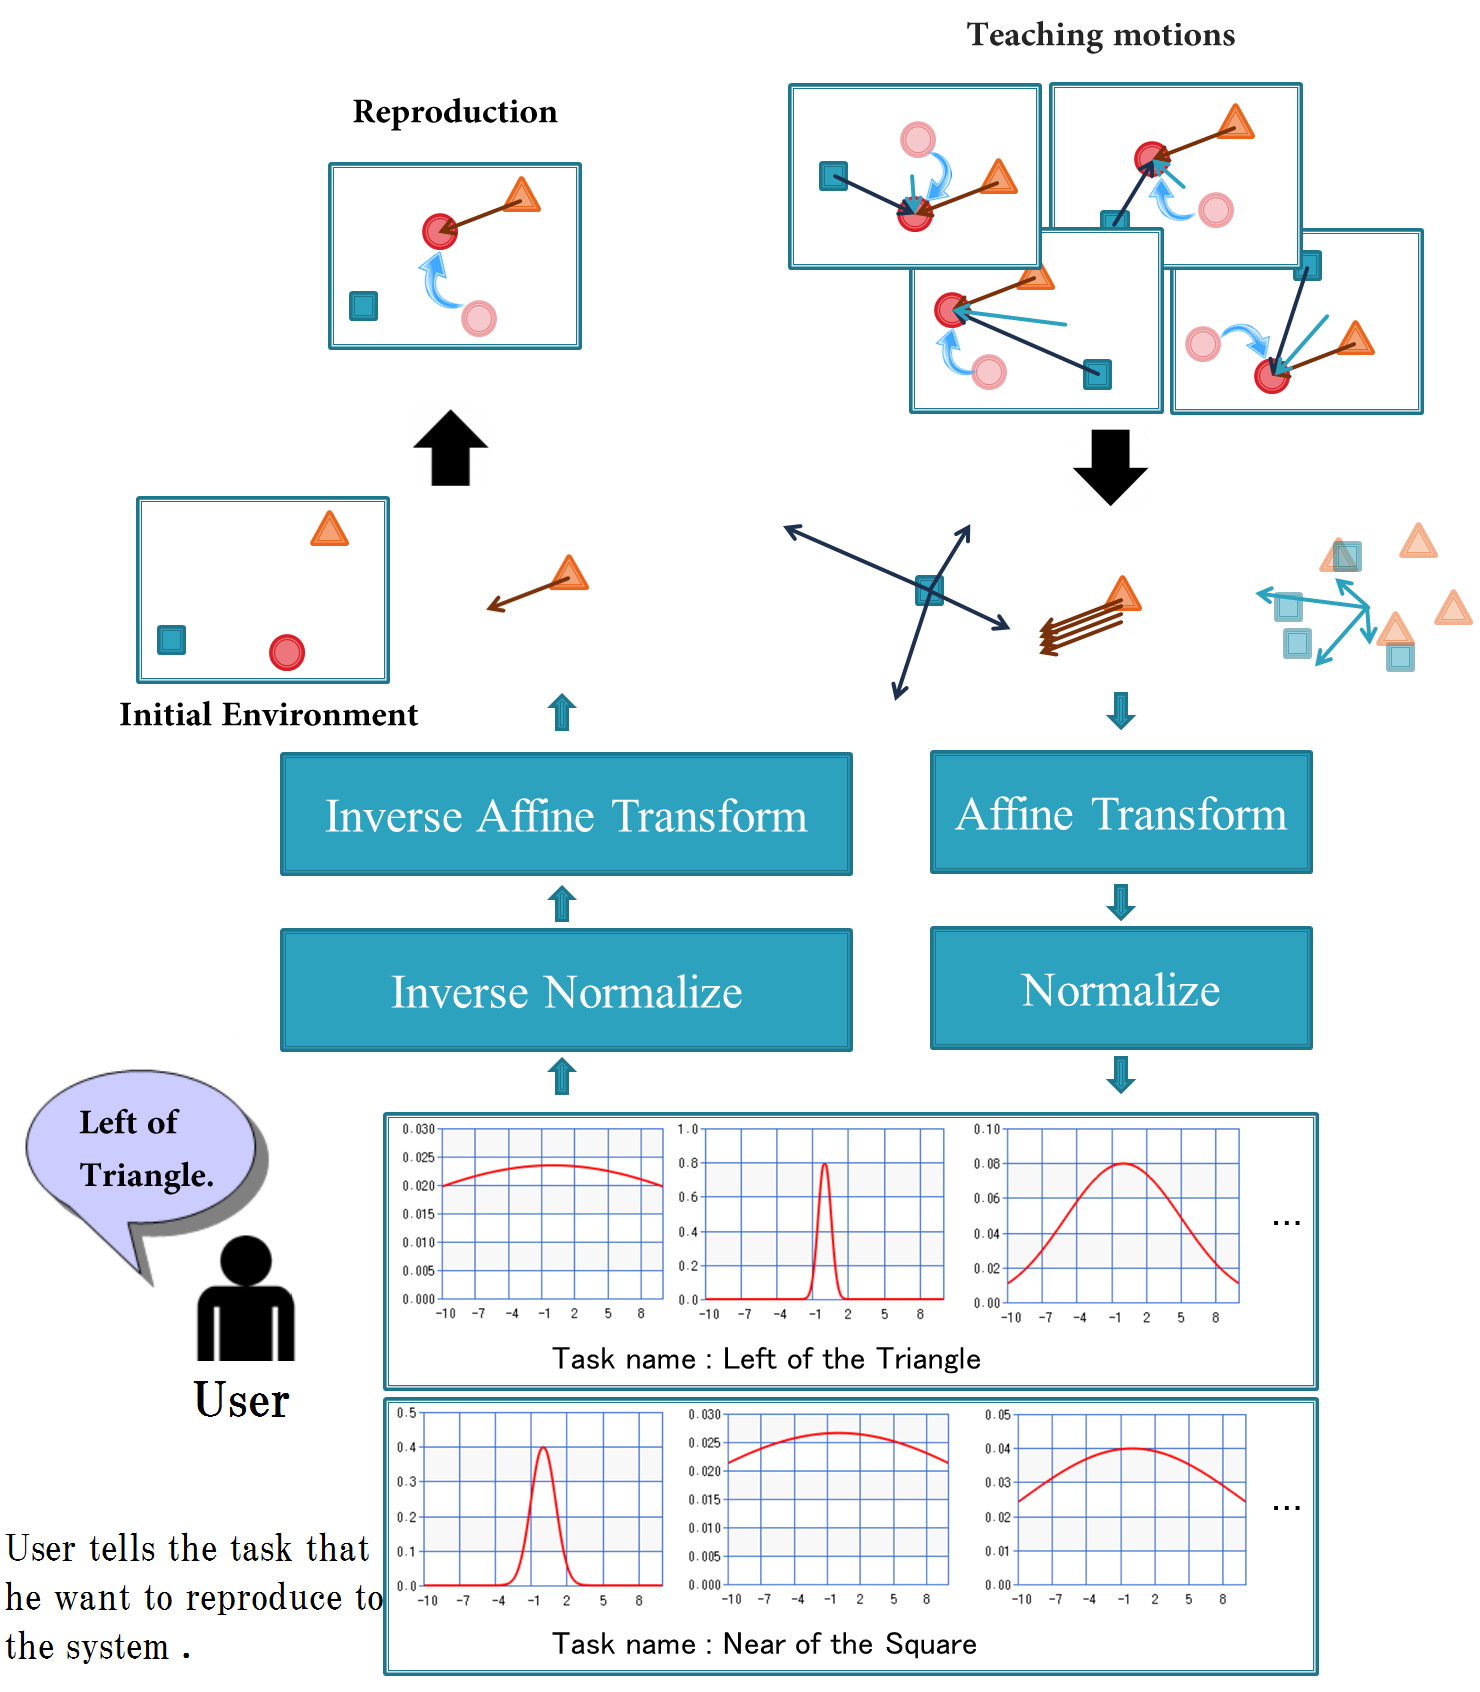
\includegraphics[width=13cm]{chart9.png} \\ %Teの基本として, \\ で緊急改行ができる。(今回の場合や行列などを除き、あまり使わない)
			\caption{動作学習と動作再現}
			\label{figure:learning_and_reproduction_model}
		\end{center}
	\end{figure}
%%%%%%%%%%%%%%%%%%%%%%%%%%%%%%%%%%%%%%%%%%%%%%%%%%%%%%%%%%%%%%%%%%%%%%%%%%%%%%%%%%%%%%%%%%%%%%%%%%%%%%%

\section{動作識別}

モデルが学習された各動作から例示動作の生起確率を計算することで、例示動作が既学習動作のうちいずれであるかを識別することが可能である。まず各動作において学習されたガウスモデルのうち分散が最小である観点を選択する。選択された観点のガウスモデルから、例示動作の目標位置が生起される確率をそれぞれ求め、生起確率が最大となるガウスモデルを持つ動作を識別結果とする。
Fig.\ref{figure:identification_model}に、提案手法における動作識別の模式図を示す。
また付録\ref{appendix3}に、動作識別のアルゴリズムの詳細を示す。
%%%%%%%%%%%%%%%%%%%%%%%%%%%%%%%%%%%%%%%%%%%%%%%%%%%%%%%%%%%%%%%%%%%%%%%%%%%%%%%%%%%%%%%%%%%%%%%%%%%%%%%
	\begin{figure}[h]
%中央ぞろえ
		\begin{center}
			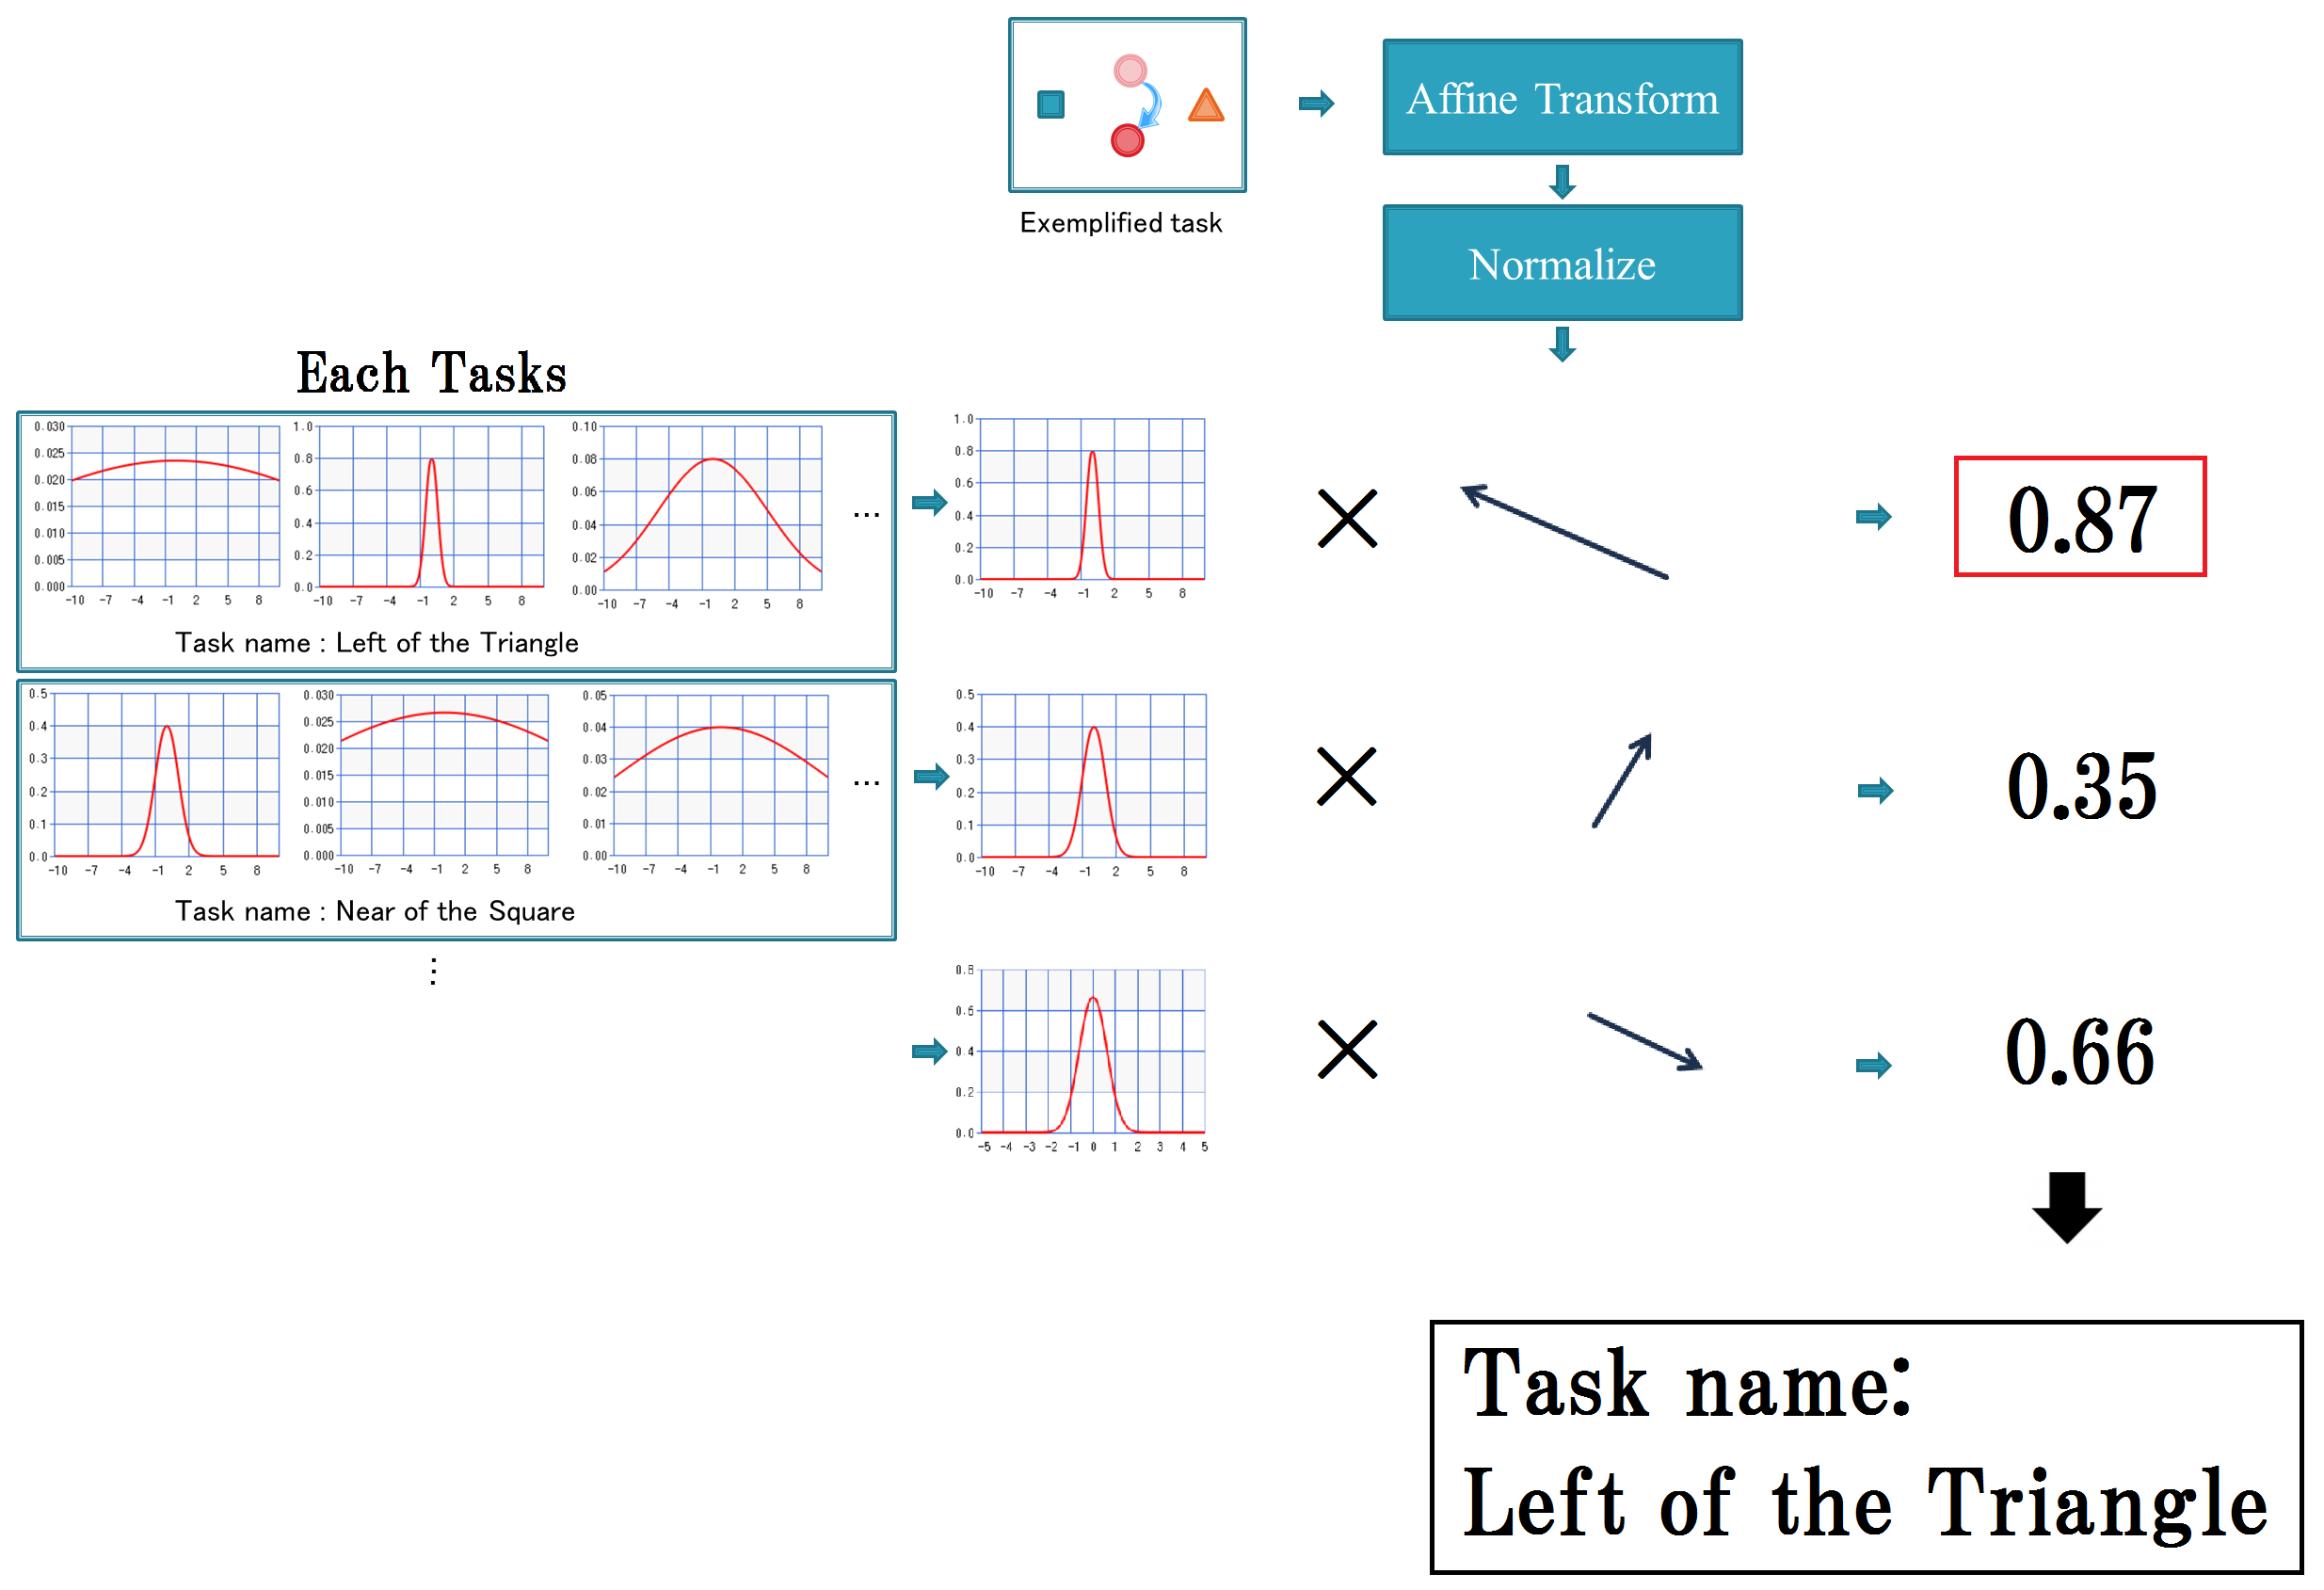
\includegraphics[width=17cm]{chart10.png} \\ %Teの基本として, \\ で緊急改行ができる。(今回の場合や行列などを除き、あまり使わない)
			\caption{動作識別}
			\label{figure:identification_model}
		\end{center}
	\end{figure}
%%%%%%%%%%%%%%%%%%%%%%%%%%%%%%%%%%%%%%%%%%%%%%%%%%%%%%%%%%%%%%%%%%%%%%%%%%%%%%%%%%%%%%%%%%%%%%%%%%%%%%%

%\chapter{Main Results}
\chapter{実験と考察}

\section{実験環境,前提}

実験環境として,2次元の有限な擬似連続空間とし,被動作対象であるトラジェクタ(赤)と,参照点となりうる4つの物体(青,橙,緑,黄)が存在する空間内での物体移動動作の学習と再現,識別を行うシミュレータ環境を準備した.被教示者にとって,空間の範囲,トラジェクタや物体の数,位置,観点の種類は既知で教示者と認識を共有しており,各動作における観点については未知であるとし,その観点を教示動作から獲得し,動作の再現と識別を行うことを目標とする.
%%%%%%%%%%%%%%%%%%%%%%%%%%%%%%%%%%%%%%%%%%%%%%%%%%%%%%%%%%%%%%%%%%%%%%%%%%%%%%%%%%%%%%%%%%%%%%%%%%%%%%%
	\begin{figure}[b]
%中央ぞろえ
		\begin{center}
			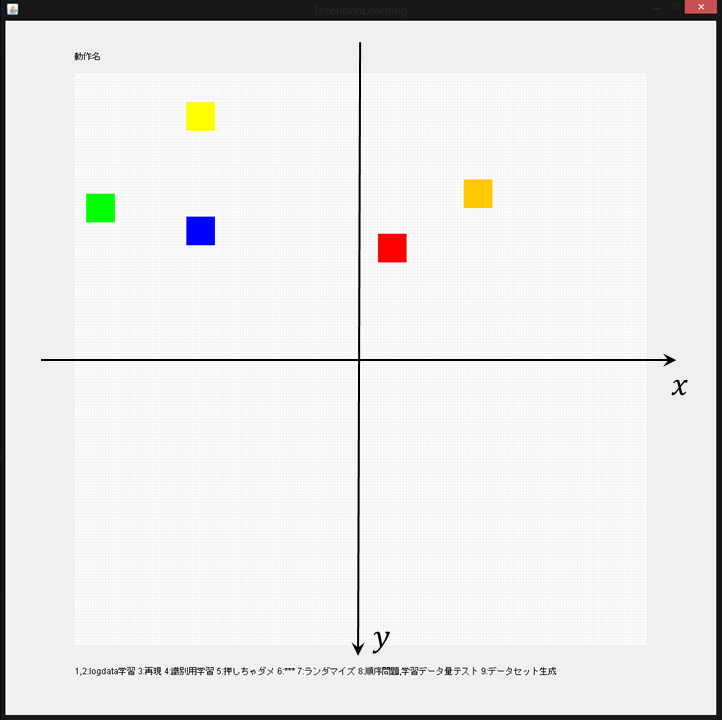
\includegraphics[width=8cm]{figure3.png} \\ %TeXの基本として, \\ で緊急改行ができる.(今回の場合や行列などを除き,あまり使わない)
			\caption{シミュレータ}
		\end{center}
	\end{figure}
%%%%%%%%%%%%%%%%%%%%%%%%%%%%%%%%%%%%%%%%%%%%%%%%%%%%%%%%%%%%%%%%%%%%%%%%%%%%%%%%%%%%%%%%%%%%%%%%%%%%%%%

\begin{table}[h]
	\caption{動作名とトラジェクタ目標位置の対応表}
	\label{table:taskname_15}
  	\begin{tabular}{|l|l|} \hline
    	動作名 & トラジェクタ目標位置\\ \hline
   	$T_{1}$ : 赤を中央に移動する & 
	$
    	\left( x_{center} , y_{center} \right)+G_{error}
    	$
    	\\
    	$T_{2}$ : 赤を青の右に移動する & 
	$
    	\left( x_{blue}+15 , y_{blue} \right)+G_{error}
    	$
%    	\\
%    	$T_{3}$ : 赤を橙の右に移動する & 
%	$
%    	\left( x_{orange}+15 , y_{orange} \right)+G_{error}
%    	$
%    	\\
%    	$T_{4}$ : 赤を緑の右に移動する & 
%	$
%    	\left( x_{green}+15 , y_{green} \right)+G_{error}
%    	$
%    	\\
%    	$T_{5}$ : 赤を黄の右に移動する & 
%	$
%    	\left( x_{yellow}+15 , y_{yellow} \right)+G_{error}
%    	$
%    	\\
%    	$T_{6}$ : 赤を青に近づける & 
%	$
%    	\left( \frac{x_{red}+x_{blue}}{2} , \frac{y_{red}+y_{blue}}{2} \right)+G_{error}
%    	$
    	\\
    	$T_{3}$ : 赤を橙に近づける & 
	$
    	\left( \frac{x_{red}+x_{orange}}{2} , \frac{y_{red}+y_{orange}}{2} \right)+G_{error}
    	$
%   	\\
%   	$T_{8}$ : 赤を緑に近づける & 
%	$
%    	\left( \frac{x_{red}+x_{green}}{2} , \frac{y_{red}+y_{green}}{2} \right)+G_{error}
%    	$
%    	\\
%    	$T_{9}$ : 赤を黄に近づける & 
%	$
%    	\left( \frac{x_{red}+x_{yellow}}{2} , \frac{y_{red}+y_{yellow}}{2} \right)+G_{error}
%    	$
%    	\\
%    	$T_{10}$ : 赤を青から遠ざける & 
%	$
%    	\left( 2x_{red}-x_{blue} , 2y_{red}-y_{blue} \right)+G_{error}
%    	$
%    	\\
%    	$T_{11}$ : 赤を橙から遠ざける & 
%	$
%    	\left( 2x_{red}-x_{orange} , 2y_{red}-y_{orange} \right)+G_{error}
%    	$
    	\\
    	$T_{4}$ : 赤を緑から遠ざける & 
	$
    	\left( 2x_{red}-x_{green} , 2y_{red}-y_{green} \right)+G_{error}
    	$
%    	\\
%    	$T_{13}$ : 赤を黄から遠ざける & 
%	$
%    	\left( 2x_{red}-x_{yellow} , 2y_{red}-y_{yellow} \right)+G_{error}
%    	$
    	\\
    	$T_{5}$ : 等間隔に赤,黄,青と並べる & 
	$
    	\left( 2x_{yellow}-x_{blue} , 2y_{yellow}-y_{blue} \right)+G_{error}
    	$
    	\\
    	$T_{6}$ : 時計回りに赤,緑,青と並べる & 
	$
	\begin{pmatrix}
        	\cos \frac{\pi}{3} & -\sin \frac{\pi}{3} \\
        	\sin \frac{\pi}{3} & \cos \frac{\pi}{3}
	\end{pmatrix}
	\begin{pmatrix}
        	x_{blue}-x_{green} \\
        	y_{blue}-y_{green}
	\end{pmatrix}
      	+
	\begin{pmatrix}
        	x_{green} \\
        	y_{green}
	\end{pmatrix}      	
	+G_{error}
    	$
    	\\ \hline
  	\end{tabular}
\end{table}
また本実験において使用した動作の,動作名とその動作におけるトラジェクタの目標位置をまとめた表をTable \ref{table:taskname_15}に示す.
ただし,Table \ref{table:taskname_15}における$x , y$は各物体の,画面中央を原点とし,画面に水平な$x$座標と,画面に垂直な$y$座標を規定した座標系(以下,画面座標)における座標成分である.また全ての物体は1辺が画面座標における10マス分の正方形とし,空間の範囲は画面座標における$x,y$軸ともに[-200 , 200]とした.$G_{error}$とは平均0のガウス分布から生起される誤差(以下,ガウス誤差)であり,分散の大きさは各実験ごとに設定する.$G_{error}$は教示誤差を表し,分散が小さいほど正確に与えられた教示動作となる.


\section{動作再現}

提案手法によって動作の学習が適切に行えていることを確認するため,
観点が被教示者にとって未知である教示動作を与え,観点を推定し動作を再現する実験を行った.
動作再現の実験にはTable \ref{table:taskname_15}の6動作を使用した.

\subsection{教示誤差と再現誤差の関係に関する実験}

動作教示時に生じた誤差(教示誤差)が,動作再現時に生じる誤差(再現誤差)にどのように影響するか調べるために,教示誤差を変化させながら再現誤差を計測する実験を行った.
教示誤差をガウス誤差の分散0.5間隔で0から20まで増やしながらそれぞれ500データ生成し,10データ1セットの一つ抜き法で再現誤差の計算を各教示誤差で計50回ずつ行った.
観点推定の成否の判定は計算結果のうち各教示誤差における標準偏差の2.896倍\footnote{付録\ref{appendix2}参照}以上の誤差が生じた再現結果を推定失敗と定めた.Fig.\ref{figure:success_rate}に,そのようにして各再現結果を成功と失敗に分けた観点推定の正答率のグラフを示す.なお,正答率の計算に用いた実験結果については付録\ref{appendix1}に示す.また付録\ref{appendix2}に,各教示誤差と再現誤差の関係と,判定基準を上記のように定められることの詳細を示す.
%%%%%%%%%%%%%%%%%%%%%%%%%%%%%%%%%%%%%%%%%%%%%%%%%%%%%%%%%%%%%%%%%%%%%%%%%%%%%%%%%%%%%%%%%%%%%%%%%%%%%%%
	\begin{figure}[h]
%中央ぞろえ
		\begin{center}
			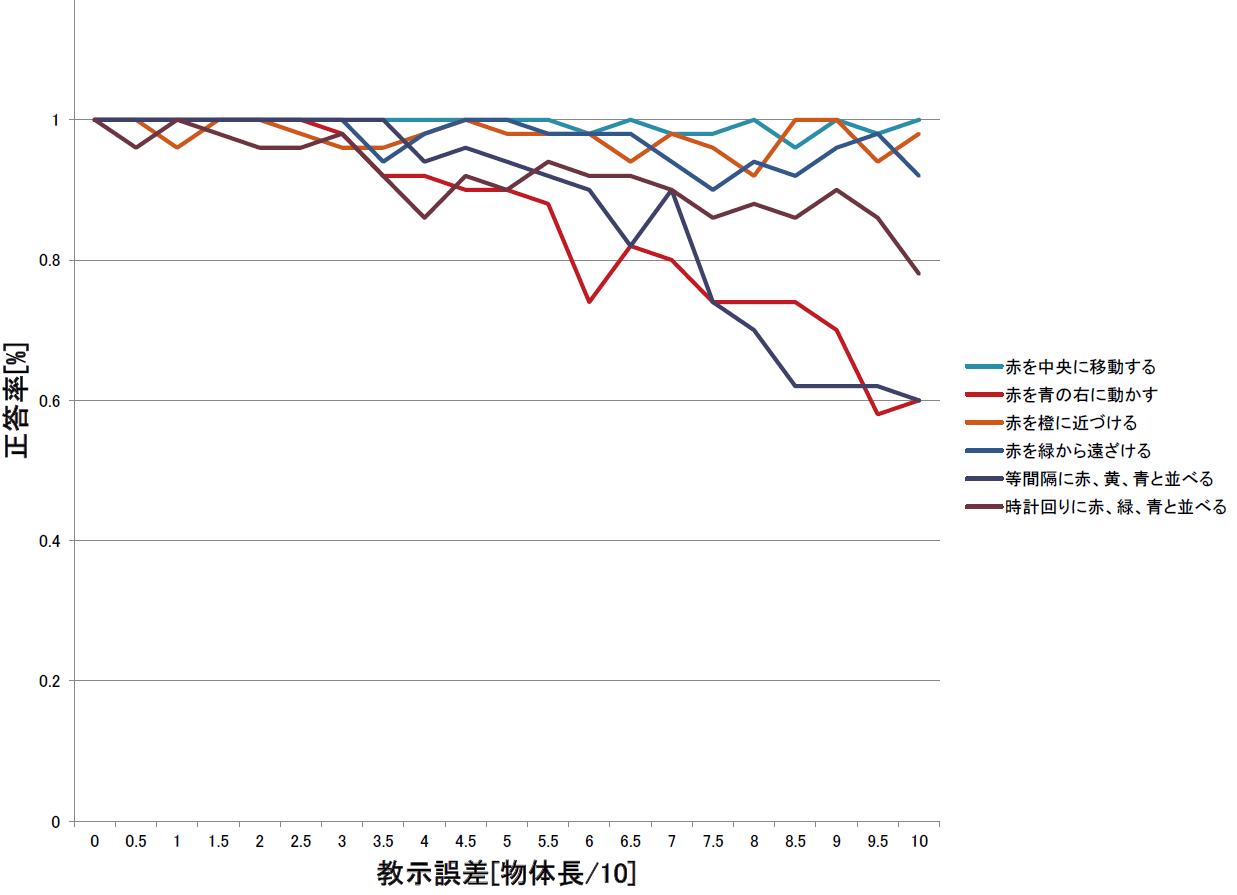
\includegraphics[width=14cm]{chart2.png} \\ %TeXの基本として, \\ で緊急改行ができる.(今回の場合や行列などを除き,あまり使わない)
			\caption{教示誤差と正答率の関係のグラフ}
			\label{figure:success_rate}
		\end{center}
	\end{figure}
%%%%%%%%%%%%%%%%%%%%%%%%%%%%%%%%%%%%%%%%%%%%%%%%%%%%%%%%%%%%%%%%%%%%%%%%%%%%%%%%%%%%%%%%%%%%%%%%%%%%%%%

Fig.\ref{figure:success_rate}から,教示誤差が十分に小さい場合に,観点の推定が適切に行えていることがわかる.また,$T_{5}$,$T_{6}$においても十分に正確な教示動作において適切に再現できていることから,複数の参照点を含む動作を適切に学習できていることがわかる.実験に使用した動作のうち,$T_{1}$,$T_{3}$,$T_{4}$の正答率が意図した状態と異なり,教示誤差の増加に無関係に再現できているが,これは学習時の遷移ベクトルの正規化関数における正規化長に依るものだと考えられる.また中央に移動する動作は中央に近づける動作とも認識できる等,適切な観点が複数存在する動作に関して誤答率が下がったとも考えられる.

\subsection{正規化長に関する考察}
\label{subsection:UNIT}
動作学習時に教示動作に適応される正規化関数$Normalize_{lk}(v)$は\ref{equation:normalize}式で表される.ここで,$unit$は正規化長を表す.正規化関数は,教示動作から得られた参照点から目標位置までの相対位置ベクトルを,あらかじめ定めた正規化長に正規化する.これは例えば物体に近づける動作など,距離的な位置関係よりも初期位置からの変化の割合が重視されるような動作や,複数の物体と特定の図形を構成するなどの相似的な配置を目標とする動作の学習に必要になる処理である.学習時,教示動作から得られるベクトル$v$の分散は\ref{equation:V_unit}式で与えられる.

\[
	V(v) = mean((F_{lk}(v))^{2}) - (mean(F_{lk}(v)))^{2}
\]
\begin{equation}
	\label{equation:V_unit}
	 = \left(\frac{unit}{| Position(L_{k})-Position(l) |}\right)^{2}(mean(v^{2}) - ((mean(v))^{2})
\end{equation}

\ref{equation:V_unit}式から,正規化後のベクトルの分散は正規化長の2乗に比例していることが分かる.動作再現時の観点の推定にガウスモデルの分散を利用しているため,正規化長の設定が動作再現の精度に関わることになる.即ち,正規化長を小さくして$k=k_{lt} , k_{gl}$におけるモデルの分散を小さくすると$k=k_{lt} , k_{gl}$である動作を優先的に学習し,正規化長を大きくして$k=k_{lt} , k_{gl}$における分散を大きくすると$k=k_{id}$である動作を優先的に学習するため,座標系に応じて再現の正答率に差異が生じたと考えられる.

\subsection{正規化長と再現誤差の関係に関する実験}

前述の実験において動作ごとに再現誤差が異なるという結果になった原因を,動作学習時に座標系$k_{lt}$,$k_{gl}$にのみ適応した正規化関数における正規化長に起因するものだという仮説を立証するため,正規化長を変化させながら再現誤差を計測する実験を行った.
正規化長を1間隔で1から50まで,4間隔で51から199まで増やしながらそれぞれ教示誤差の分散10で500データ生成し,10データ1セットの一つ抜き法で再現誤差の計算を描く教示誤差で計50回ずつ行った.
観点推定の成否の判定は同様に計算結果のうち教示誤差における標準偏差の2.896倍\footnote{付録\ref{appendix2}参照}以上の誤差が生じた再現結果を推定失敗と定めた.Fig.\ref{figure:success_rate_for_UNIT}に,そのようにして各再現結果を成功と失敗に分けた観点推定の正答率のグラフを示す.
\ref{subfigure:unit_b}は使用した6動作のうち,座標系が$k_{id}$であることが期待される動作である$T_{1}$と$T_{2}$の結果を表したものである.結果から,$T_{2}$に関しては仮説通り,正規化長が増加するにつれて再現精度が向上していることが分かる.
\ref{subfigure:unit_c}は座標系が$k_{lt}$であることが期待される動作である$T_{3}$と$T_{4}$の結果を表したものである.結果から,仮説通り,正規化長が増加するにつれて再現精度が低下していることが分かる.
座標系が$k_{gl}$であることが期待される動作である$T_{5}$と$T_{6}$も同様に\ref{subfigure:unit_d}に示された結果から,仮説通り,正規化長が増加するにつれて再現精度が低下していることが分かる.また$k_{gl}$の動作が$k_{lt}$の動作よりも正規化長の影響を大きく受けているのは,\ref{equation:V_unit}式の分母$| Position(L_{k})-Position(l) |$の値が,参照点とトラジェクタ初期位置の距離を表している$k_{lt}$に対し,重心と構成参照点の距離を表している$k_{gl}$の方が比較的に小さい値となる場合が多いことが原因と考えられる.
$T_{1}$が正規化長に関わらず再現精度を維持しているのは,前述のとおり$T_{1}$が$k_{id}$,$k_{lt}$両方の観点で推定できるためだと考えられる.すなわち,正規化長が小さい場合には$k_{lt}$として,大きい場合には$k_{id}$として学習されることが可能であるため,常に高い再現精度を維持していると考えられる.

%%%%%%%%%%%%%%%%%%%%%%%%%%%%%%%%%%%%%%%%%%%%%%%%%%%%%%%%%%%%%%%%%%%%%%%%%%%%%%%%%%%%%%%%%%%%%%%%%%%%%%%
\begin{figure}[h]
	\centering
	\begin{minipage}[t]{.49\textwidth}
		\centering
		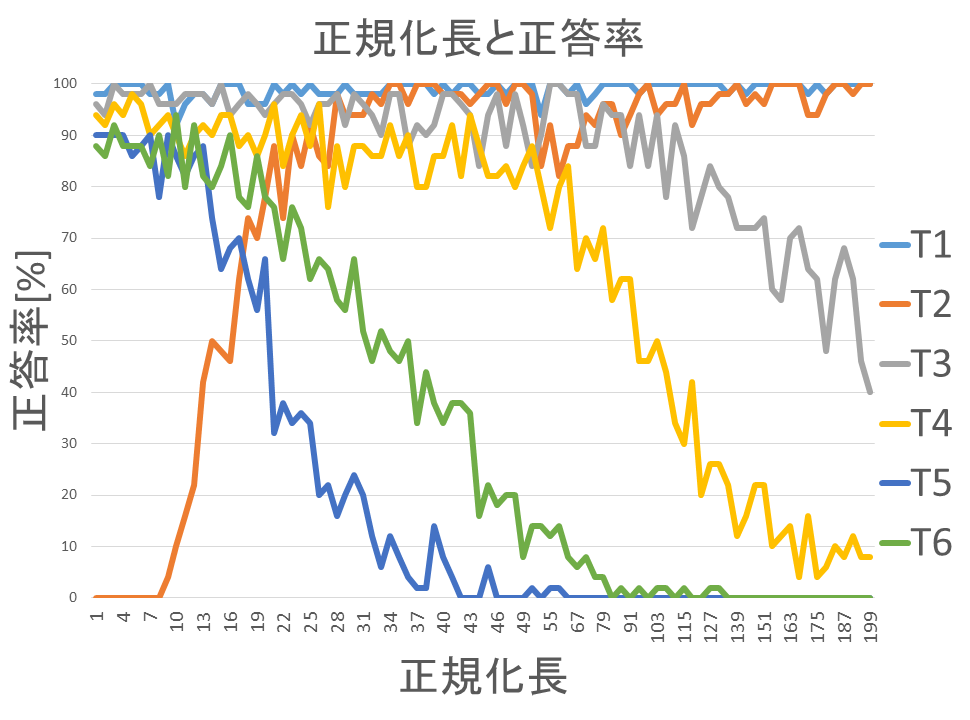
\includegraphics[width=7.5cm]{chart11_a.png} \\ %TeXの基本として, \\ で緊急改行ができる.(今回の場合や行列などを除き,あまり使わない)
		\subcaption{全動作}
		\label{subfigure:unit_a}    
	\end{minipage}
	\begin{minipage}[t]{.49\textwidth}
		\centering
		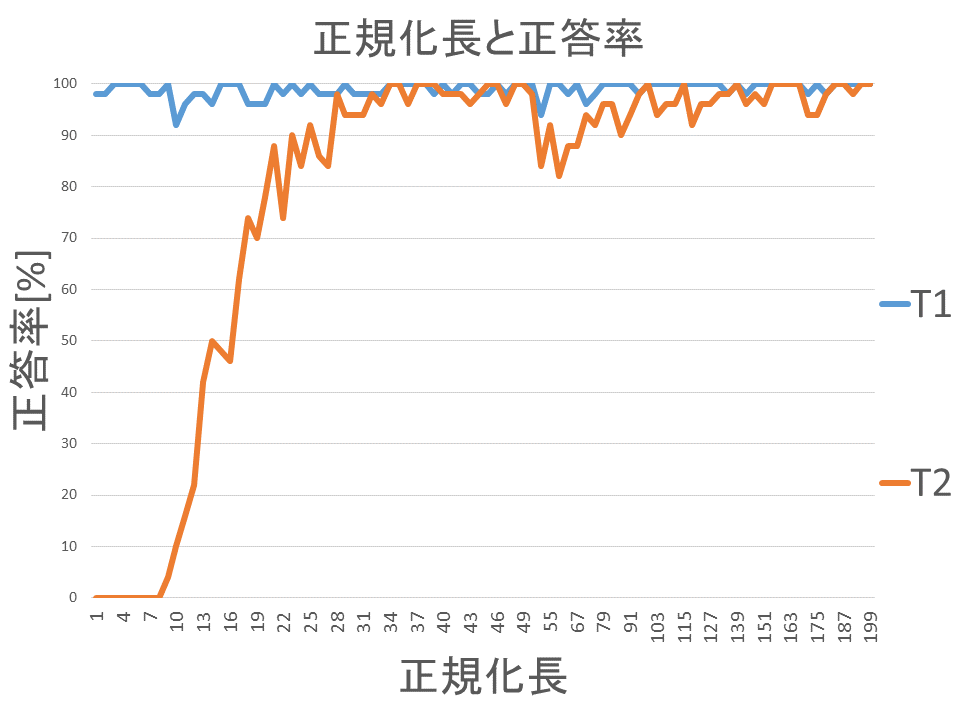
\includegraphics[width=7.5cm]{chart11_b.png} \\ %TeXの基本として, \\ で緊急改行ができる.(今回の場合や行列などを除き,あまり使わない)
		\subcaption{$T_{1}$,$T_{2}$}
		\label{subfigure:unit_b}
	\end{minipage}
	\begin{minipage}[t]{.49\textwidth}
		\centering
		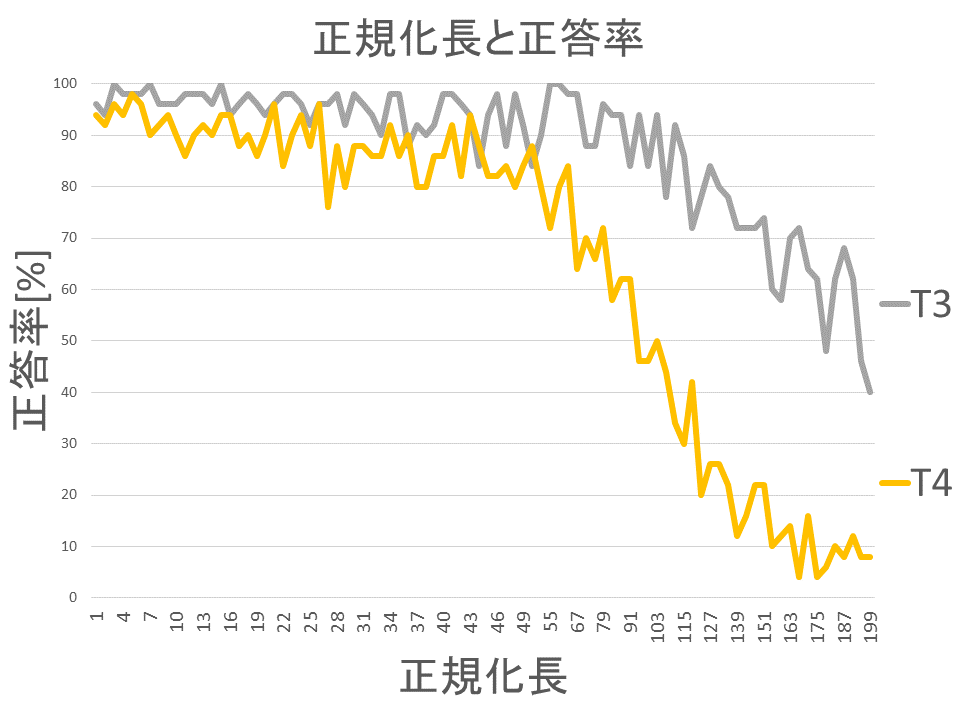
\includegraphics[width=7.5cm]{chart11_c.png} \\ %TeXの基本として, \\ で緊急改行ができる.(今回の場合や行列などを除き,あまり使わない)
		\subcaption{$T_{3}$,$T_{4}$}
		\label{subfigure:unit_c}
	\end{minipage}
	\begin{minipage}[t]{.49\textwidth}
		\centering
		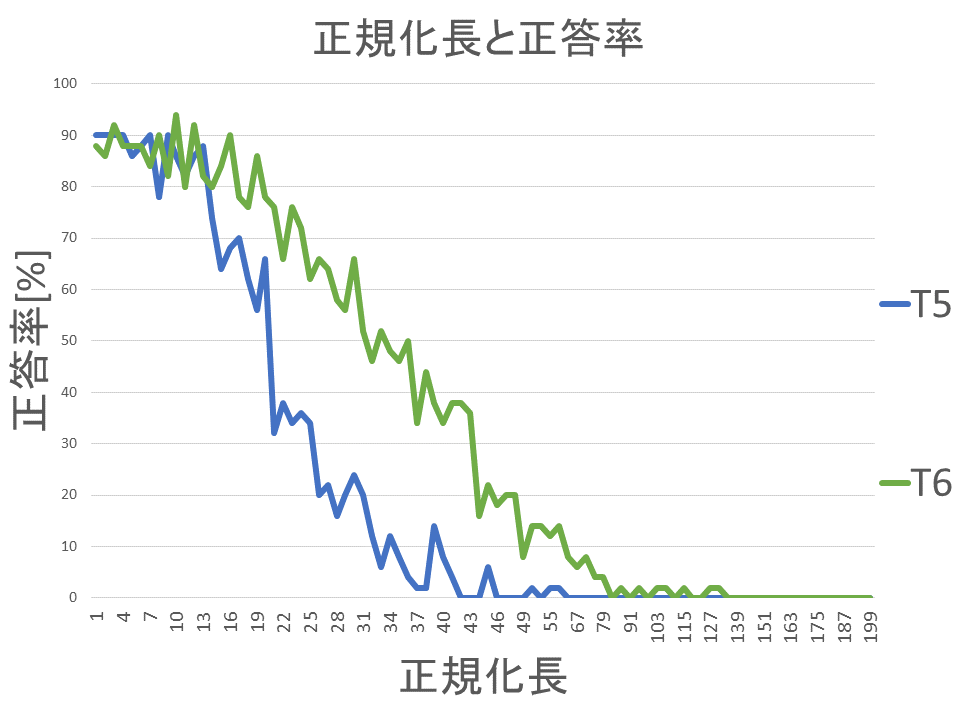
\includegraphics[width=7.5cm]{chart11_d.png} \\ %TeXの基本として, \\ で緊急改行ができる.(今回の場合や行列などを除き,あまり使わない)
		\subcaption{$T_{5}$,$T_{6}$}
		\label{subfigure:unit_d}
	\end{minipage}
	\caption{正規化長と正答率の関係のグラフ}
	\label{figure:success_rate_for_UNIT}
\end{figure}
%%%%%%%%%%%%%%%%%%%%%%%%%%%%%%%%%%%%%%%%%%%%%%%%%%%%%%%%%%%%%%%%%%%%%%%%%%%%%%%%%%%%%%%%%%%%%%%%%%%%%%%


\section{動作識別}

動作名が未知である例示動作を与え,それが既学習動作および未学習動作のうちいずれであるかを推定する実験を行った.
既学習動作はTable \ref{table:taskname_15}の6動作に,各動作に関して変位が等しく参照点を変えて生成した9動作を加えた計15動作とした.また未学習動作として,空間上の不特定の点へトラジェクタを移動する動作も識別対象とした.
各動作において教示動作として分散3のガウス誤差を持つ30データを生成し学習を行った.例示動作は動作再現実験と同様の6動作および未学習動作を使用し,学習済みである6動作はそれぞれ分散10のガウス誤差を持つ100データを生成してテストを行った.未学習動作の判定閾値はガウス分布における95\%信頼区間とした.Table \ref{table:result}に各例示動作の識別正答率を示す.
Table \ref{table:result}より,学習済みの動作に関して例示動作の識別が適切に行えていることがわかる.また,未学習動作に関しても高い識別精度を示し,既学習動作と未学習動作を適切に区別できていることが分かる.
誤識別が生じた初期環境と例示動作の例をFig.\ref{figure:failure}に示す.Fig.\ref{subfigure:failure1}は赤を橙に近づける例示動作だが,赤を緑から遠ざける動作だと誤って識別されている.誤識別が生じた例示動作に関しては,ほとんどがこのように人間にとっても適切な動作が判別し難いものであった.またFig.\ref{subfigure:failure2}は唯一既学習動作である例示動作を未学習動作と誤識別した例である.Fig.\ref{subfigure:failure2}が未学習動作だと誤識別された理由については,初期の赤と橙の位置関係に対して小さくない例示誤差が付与し正答が導かれなかったことに加え,他物体が最終位置から遠く離れており,既学習動作であるいずれの動作とも大きく異なったためであると考えられる.

\begin{table}[h]
	\caption{動作識別の正答率}
	\label{table:result}
	\centering
  	\begin{tabular}{|l|l|} \hline
    	動作名 & 正答率\\ \hline
   	赤を中央に移動する 		& 0.97
    	\\
    	赤を青の右に移動する 		& 0.98
    	\\
    	赤を橙に近づける 			& 0.93
    	\\
    	赤を緑から遠ざける 			& 0.97
    	\\
    	等間隔に赤,黄,青と並べる 	& 0.97
    	\\
    	時計回りに赤,緑,青と並べる 	& 0.98
    	\\
    	未学習動作				& 0.90
    	\\ \hline
  	\end{tabular}
\end{table}

%%%%%%%%%%%%%%%%%%%%%%%%%%%%%%%%%%%%%%%%%%%%%%%%%%%%%%%%%%%%%%%%%%%%%%%%%%%%%%%%%%%%%%%%%%%%%%%%%%%%%%%
\begin{figure}[h]
	\centering
	\begin{minipage}[t]{.47\textwidth}
		\centering
		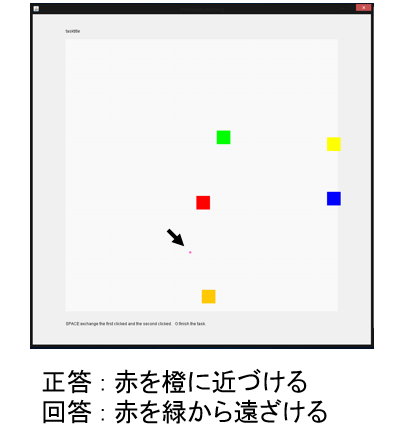
\includegraphics[width=7cm]{figure4_a.png} \\ %TeXの基本として, \\ で緊急改行ができる.(今回の場合や行列などを除き,あまり使わない)
		\subcaption{誤識別の例1}
		\label{subfigure:failure1}    
	\end{minipage}
	\begin{minipage}[t]{.47\textwidth}
		\centering
		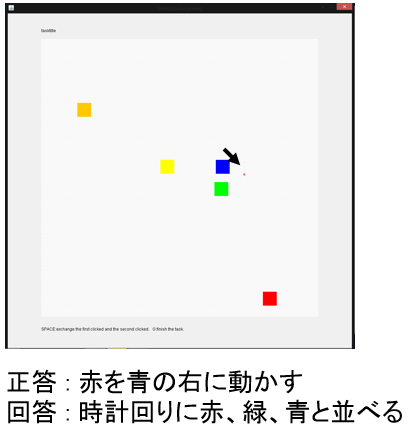
\includegraphics[width=7cm]{figure4_b.png} \\ %TeXの基本として, \\ で緊急改行ができる.(今回の場合や行列などを除き,あまり使わない)
		\subcaption{誤識別の例2}
		\label{subfigure:failure2}
	\end{minipage}
	\caption{誤識別の例}
	\label{figure:failure}
\end{figure}
%%%%%%%%%%%%%%%%%%%%%%%%%%%%%%%%%%%%%%%%%%%%%%%%%%%%%%%%%%%%%%%%%%%%%%%%%%%%%%%%%%%%%%%%%%%%%%%%%%%%%%%


%\chapter{Conclusion}
\chapter{結論}

\section{結びと課題}

本研究では,物体移動動作において,教示者の動作を考えうる観点の候補ごとの変換を施した上でベクトルの生起確率モデルとして学習することで,教示者の動作意図を把握した目標位置の推定を行うことを目標としていた.その上で参照点の候補に参照点間の重心位置を含めることで,複数の参照点間の位置関係を考慮した物体移動動作の学習を可能にした.提案手法の課題として,全ての重心位置を参照点とすることで考慮する観点の数が物体数に対して指数関数的に増加してしまう点が挙げられる.また,今回扱った各物体の位置情報以外に,形や角度,色などの一般的な特徴量を考慮した観点推定が可能になれば,より高度な動作意図を理解することができると考えられるが,その場合本研究で扱った単純な空間座標としての変換よりも一般的で高次な座標系を設定する必要がある.それらの問題を解決する方法として,ディープラーニングの手法を用いて教示データから自動的に必要な参照点や座標系を導出することが可能になれば,より広範囲で一般的な学習手法になると考えられる.
将来的には,今回の方法で獲得した最終位置をもとに,動作軌跡の認識,推定と再生成を行いたい.
また,気が利くロボットの実現に向けて,動作教示の利便性を高めるために,多量に与えられた教示動作のうち学習に適した教示のみを選択して学習することで学習効率を上げる方法や,教示中に誤った動作を認識させてしまった場合,誤教示と判断できる動作を自動的に排除して学習を行う方法についての考察も行いたい.


%\chapter*{Acknowledgements}
%\addchapter{Acknowledgements}
\chapter*{謝辞}
\addchapter{謝辞}

皆さんに感謝.皆さんに感謝.皆さんに感謝.皆さんに感謝.
皆さんに感謝.皆さんに感謝.皆さんに感謝.皆さんに感謝.
皆さんに感謝.皆さんに感謝.皆さんに感謝.皆さんに感謝.

%\addchapter{References}
\addchapter{参考文献}
\begin{thebibliography}{9}% 文献数が10未満の時 {9},10~99の時 {99}
\bibitem{sugiura}
杉浦孔明, et al. "Learning, generation and recognition of motions by reference-point-dependent probabilistic models." Advanced Robotics 25.6-7 (2011): 825-848.

\bibitem{dong}
Dong, Shuonan, and Brian Williams. "Learning and recognition of hybrid manipulation motions in variable environments using probabilistic flow tubes." International Journal of Social Robotics 4.4 (2012): 357-368.

\bibitem{nakaoka}
中岡慎一郎, et al. "シンボリックな動作記述を用いた舞踊動作模倣ロボットの実現." 電子情報通信学会技術研究報告. PRMU パターン認識・メディア理解 103.390 (2003): 55-60.

\bibitem{Koenemann}
Koenemann, Jonas, Felix Burget, and Maren Bennewitz. "Real-time imitation of human whole-body motions by humanoids." Robotics and Automation (ICRA), 2014 IEEE International Conference on. IEEE, 2014.

\bibitem{schaal} 
Schaal, Stefan. "Dynamic movement primitives-a framework for motor control in humans and humanoid robotics." Adaptive Motion of Animals and Machines. Springer Tokyo, 2006. 261-280.

\bibitem{imitation1} 
Argall, Brenna D., et al. "A survey of robot learning from demonstration." Robotics and autonomous systems 57.5 (2009): 469-483.

\bibitem{imitation2}
臼井和廉, 波多野拓貴, and 高橋泰岳. "人間による呈示動作のバイアスを用いた人型ロボットの模倣学習." ファジィシステムシンポジウム講演論文集 29 (2013): 836-841.

\bibitem{imitation3}
Eppner, Clemens, et al. "Imitation learning with generalized task descriptions." Robotics and Automation, 2009. ICRA'09. IEEE International Conference on. IEEE, 2009.

\bibitem{imitation4}
Khansari-Zadeh, S. Mohammad, and Aude Billard. "Learning stable nonlinear dynamical systems with gaussian mixture models." Robotics, IEEE Transactions on 27.5 (2011): 943-957.

\end{thebibliography}



\appendix
%\chapter{Proof of Theorem 1}\label{appendix1}
\chapter{提案手法のアルゴリズム}\label{appendix3}

\section{動作学習のアルゴリズム}

与えられた教示動作を用いて,各観点における確率モデルを更新し,学習を行う.Algorithm \ref{algorithm1}に,提案手法の学習のアルゴリズムを示す.
	\begin{algorithm}[b]
		\caption{ Learning algorithm of the proposed method}
		\label{algorithm1}
		\begin{algorithmic}
			\REQUIRE
				$N$ : the number of training data \\
				$M$ : the number of reference points , 
				$O$ : the number of objects \\
				$D = \{D_{1} , D_{2} , \ldots , D_{N}\}$ : training dataset \\
				$L = \{l_{1} , l_{2} , \ldots , l_{M}\}$ : the candidates of the reference point \\
				$K = \{k_{id} , k_{lt} , k_{gl}\}$ : coordinate systems \\
				$V = <L , K>$ : the candidates of the viewpoints \\
				$μ_{lk}$ : mean of the Probabilistic model of $<l , k>$ \\
				$Q_{lk}$ : mean-square of the Probabilistic model of $<l , k>$ \\
				$σ_{lk}$ : variance of the Probabilistic model of $<l , k>$ \\
				$Transform_{lk}(v)$ : Affine transfomation , 
				$Normalize_{lk}(v)$ : Normalization
		\end{algorithmic}
		\begin{algorithmic}[1]
			\STATE $M \leftarrow 2^{O}$
			
			\FOR{$n=1$ to $N$}
				\STATE $d \leftarrow D_{n}$
				\FOR{$m=1$ to $M$}
					\FOR{all $k ∈K$}
						\STATE $d_{l_{m}k} \leftarrow Normalize_{l_{m}k}(Transform_{l_{m}k}(d))$
						\STATE $μ_{l_{m}k} \leftarrow \frac{n-1}{n}μ_{l_{m}k} + \frac{1}{n}d_{l_{m}k}$
						\STATE $Q_{l_{m}k} \leftarrow \frac{n-1}{n}Q_{l_{m}k} + \frac{1}{n}(d_{l_{m}k})^2$
						\STATE $σ_{l_{m}k} \leftarrow Q_{l_{m}k} - (μ_{l_{m}k})^2$
					\ENDFOR
				\ENDFOR
			\ENDFOR
		\end{algorithmic}
	\end{algorithm}
ここで,$k_{id} , k_{lt} , k_{gl}$は座標系を表し,それぞれ画面に平行,参照点からトラジェクタの初期位置方向,参照点から重心の構成物体方向とする.参照点が複数の物体の重心でない場合,$k_{gl}$は考慮しない.


\section{動作再現のアルゴリズム}

教示動作から学習された各観点における確率モデルを用いて,異なる初期環境での動作再現を行う.Algorithm \ref{algorithm2}に,提案手法の動作再現のアルゴリズムを示す.
	\begin{algorithm}[h]
		\caption{ Reproduction algorithm of the proposed method}
		\label{algorithm2}
		\begin{algorithmic}
			\REQUIRE
				$M$ : the number of reference points \\ 
				$L = \{l_{1} , l_{2} , \ldots , l_{M}\}$ : the candidates of the reference point \\
				$K = \{k_{id} , k_{lt} , k_{gl}\}$ : coordinate systems \\
				$V = <L , K>$ : learned models of the viewpoints \\
				$μ_{lk}$ : mean of the Probabilistic model of $<l , k>$ \\
				$Q_{lk}$ : mean-square of the Probabilistic model of $<l , k>$ \\
				$σ_{lk}$ : variance of the Probabilistic model of $<l , k>$ \\
				$Transform_{lk}(v)$ : Affine transfomation , 
				$Normalize_{lk}(v)$ : Normalization \\
				$Position(l)$ : Position of the reference point $l$
		\end{algorithmic}
		\begin{algorithmic}[1]
			\STATE $<l_{max} , k_{max}> \leftarrow <l_{1} , k_{1}>$
			\FOR{all $<l , k>∈V$}
				\IF{$σ_{lk} < σ_{l_{max}k_{max}}$}
					\STATE $<l_{max} , k_{max}> \leftarrow <l , k>$
				\ENDIF
			\ENDFOR
			\STATE $d \leftarrow Transform^{-1}(Normalize^{-1}(μ_{l_{max}k_{max}}))$
			\STATE $d \leftarrow d + Position(l_{max})$
		\end{algorithmic}
	\end{algorithm}


\section{動作識別のアルゴリズム}

モデルが学習された各動作から例示動作の生起確率を計算することで,例示動作が既学習動作のうちいずれであるか識別を行う.Algorithm \ref{algorithm3}に,提案手法の動作識別のアルゴリズムを示す.
	\begin{algorithm}[h]
		\caption{ Identification algorithm of the proposed method}
		\label{algorithm3}
		\begin{algorithmic}
			\REQUIRE
				$x_{input}$ : the destination of the exemplified task \\ 
				$M$ : the number of reference points , 
				$S$ : the number of learned tasks \\
				$L = \{l_{1} , l_{2} , \ldots , l_{M}\}$ : the candidates of the reference point \\
				$K = \{k_{id} , k_{lt} , k_{gl}\}$ : coordinate systems \\
				$T = \{t_{1} , t_{2} , \ldots t_{S}\}$ : learned tasks \\
				$V_{t} = <L_{t} , K_{t}>$ : learned models of the viewpoints in the task $t$\\
				$μ_{lk}$ : mean of the Probabilistic model of $<l , k>$ \\
				$Q_{lk}$ : mean-square of the Probabilistic model of $<l , k>$ \\
				$σ_{lk}$ : variance of the Probabilistic model of $<l , k>$ \\
				$Transform_{lk}(v)$ : Affine transfomation , 
				$Normalize_{lk}(v)$ : Normalization \\
				$Probability(<i , k> , x)$ : Probability that $x$ is generated from $<l , k>$
		\end{algorithmic}
		\begin{algorithmic}[1]
			\STATE $t_{max} \leftarrow t_{1}$
			\STATE $<l_{max} , k_{max}> \leftarrow <l_[1] , k_[1]>$
			
			\FOR{all $t∈T$}
				\STATE $<l_{max}^{t} , k_{max}^{t}> \leftarrow <l_{1}^{t} , k_{1}^{t}>$
				\FOR{all $<l^{t} , k^{t}>∈V_{t}$}
					\IF{$σ_{l^{t}k^{t}} < σ_{l_{max}^{t}k_{max}^{t}}$}
						\STATE $<l_{max}^{t} , k_{max}^{t}> \leftarrow <l^{t} , k^{t}>$
					\ENDIF
				\ENDFOR
				\IF{$Probability(<l_{max}^{t} , k_{max}^{t}> , v_{input}) > Probability(<l_{max} , k_{max}> , v_{input})$}
					\STATE $<l_{max} , k_{max}> \leftarrow <l_{max}^{t} , k_{max}^{t}>$
					\STATE $t_{max} \leftarrow t$
				\ENDIF
			\ENDFOR
		\end{algorithmic}
	\end{algorithm}

\clearpage
\chapter{動作再現実験における実験結果}\label{appendix1}

動作の再現実験における,教示誤差と再現誤差の関係を図\ref{figure:errors}に示す.
ここで,横軸は教示誤差の分散,縦軸は再現誤差の標準偏差を表す.
各教示誤差において,教示動作からの学習,再現を行った際の再現誤差を50回ずつ実験を行った.適切な観点が選択されている場合,教示誤差と再現誤差の分散が等しくなることが期待される.即ち各グラフにおいて教示誤差$t$,再現誤差$r$に関して,
\[
	r = \sqrt{t}
\]
という関係が満たされていることが期待される.実際のグラフ中には,無理関数に従うように見える結果と,相関が見られ難い結果が存在している.これらの違いと判別基準については付録\ref{appendix2}で説明する.

%%%%%%%%%%%%%%%%%%%%%%%%%%%%%%%%%%%%%%%%%%%%%%%%%%%%%%%%%%%%%%%%%%%%%%%%%%%%%%%%%%%%%%%%%%%%%%%%%%%%%%%
	\begin{figure}
%中央ぞろえ
		\begin{center}
			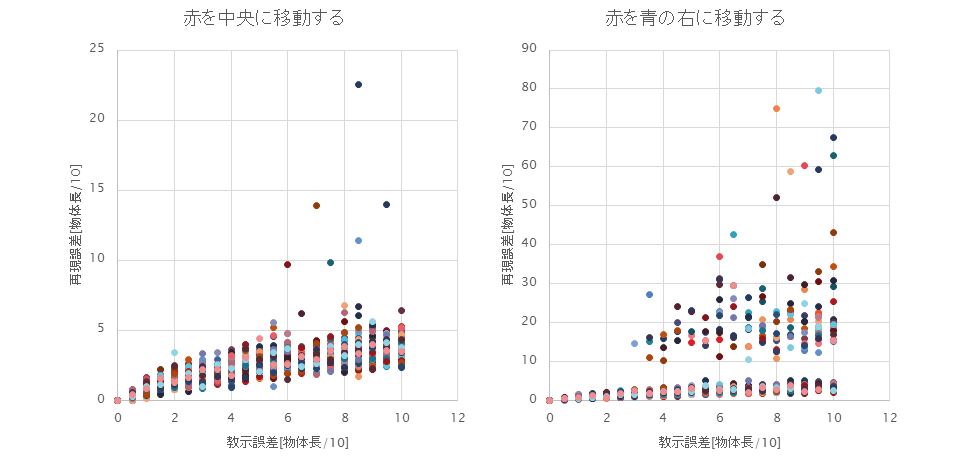
\includegraphics[width=15.5cm]{chart6.png} \\ %eXの基本として, \\ で緊急改行ができる.(今回の場合や行列などを除き,あまり使わない)
			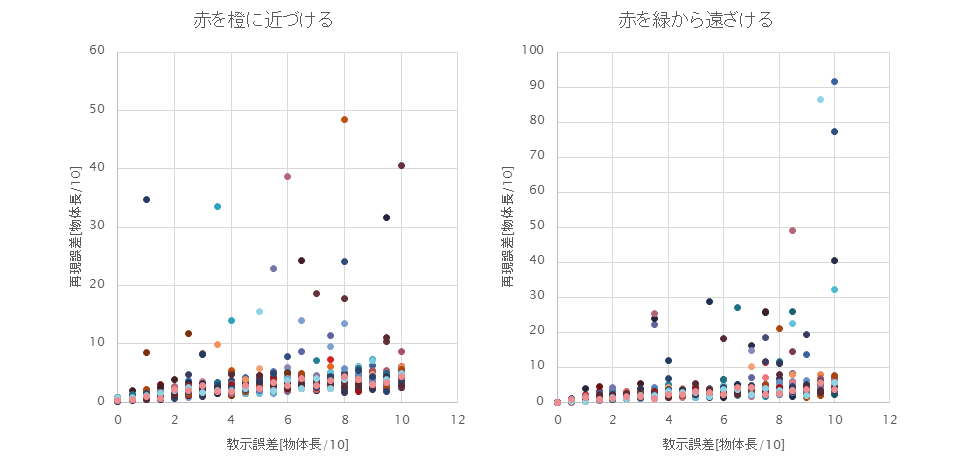
\includegraphics[width=15.5cm]{chart7.png} \\ %eXの基本として, \\ で緊急改行ができる.(今回の場合や行列などを除き,あまり使わない)
			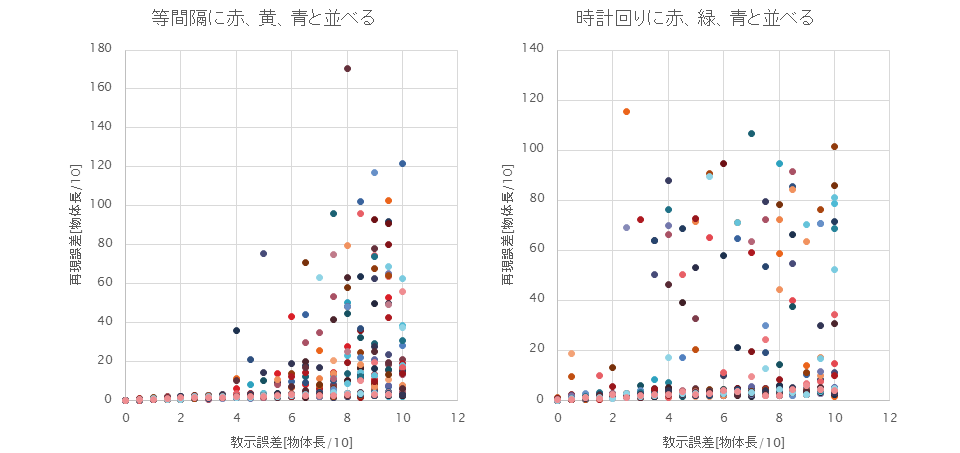
\includegraphics[width=15.5cm]{chart8.png} \\ %eXの基本として, \\ で緊急改行ができる.(今回の場合や行列などを除き,あまり使わない)
			\caption{教示誤差と再現誤差}
			\label{figure:errors}
		\end{center}
	\end{figure}
%%%%%%%%%%%%%%%%%%%%%%%%%%%%%%%%%%%%%%%%%%%%%%%%%%%%%%%%%%%%%%%%%%%%%%%%%%%%%%%%%%%%%%%%%%%%%%%%%%%%%%%


\chapter{動作再現における観点推定の成否の判定}\label{appendix2}

教示動作から学習したモデルを用いた動作再現を行う際,教示動作自体に誤差が含まれている場合,一つ抜き法によるテスト時に使用するデータも教示動作の一つであるために必然的に誤差が生じる.そのため一つ抜き法により計算された再現誤差が教示誤差に依るものなのか誤学習に依るものなのかを区別する基準が必要である.ここでは正規分布から生成された誤差を含む教示動作から適切に学習された場合に再現誤差も正規分布に従うことを示し,正規分布の性質から観点推定の成否の基準値を設定する.
まず,適切な観点(原点となる参照点と座標系)からの$N$回分の各教示動作における目標位置$Θ=\{θ_{1} , θ_{2} , \ldots , θ_{N}\}$に対し,$Θ$を用いた一つ抜き法による評価値を次のように求める.
	\begin{equation}
		\label{CrossVaridation}
		Cr(Θ) = \frac{1}{N} \sum_{n=1}^{N} F(θ_{n} | Θ \backslash θ_{n})
	\end{equation}
ここで\ref{CrossVaridation}式の右辺$F(θ_{n} | Θ \backslash θ_{n})$は,$θ_{n}$を除く$Θ$を用いて学習し再現を行った結果の目標位置と$θ_{n}$の誤差を表す.動作再現は選択された観点に割り当てられた正規分布の平均を出力するので,
	\begin{equation}
		\label{F}
		F(θ_{n} | Θ \backslash θ_{n}) = |θ_{n} - mean(Θ \backslash θ_{n})| = |\frac{N}{N-1}(θ_{n} - mean(Θ))|
	\end{equation}
である.ただし$mean(A)$はAの平均とする.\ref{F}式を\ref{CrossVaridation}に代入すると
	\begin{equation}
		\label{Cr2}
		Cr(Θ) = \frac{1}{N} \sum_{n=1}^{N}  |\frac{N}{N-1}(θ_{n} - mean(Θ))|
		 = \frac{N}{N-1}\frac{1}{N}  \sum_{n=1}^{N}  |(θ_{n} - mean(Θ))| 
	\end{equation}
と整理できる.ここで\ref{Cr2}式の右辺$|(θ_{n} - mean(Θ))|$は$θ_{n}$の持つガウス誤差と等しいので,
	\begin{equation}
		\label{Cr3}
		mean(Cr(Θ)) = \frac{N}{N-1} * mean(\frac{1}{N}  \sum_{n=1}^{N}  |(θ_{n} - mean(Θ))| )
		 = \frac{N}{N-1} * mean(|G_{error}|)
	\end{equation}
となる.$2\int_{0}^{\infty}G_{error}(v)dv = \sqrt{\frac{2}{\pi}}σ$であることから,$Cr(Θ)$の平均は
	\begin{equation}
		\label{Cr4}
		mean(Cr(Θ)) = \frac{N}{N-1}\sqrt{\frac{2}{\pi}}σ
	\end{equation}
と求められる.ただし$σ$はガウス誤差の分散である.同様に,
	\begin{equation}
		\label{Cr^2_1}
		mean(Cr(Θ)^2) = \left(\frac{N}{N-1}\right)^2 * mean(|G_{error}|^2) 
		= 2\int_{0}^{\infty}\frac{x^2}{\sqrt{2\pi}σ}e^{-\frac{x^2}{2σ^2}}dx
	\end{equation}
であり,これを計算することで,
	\begin{equation}
		\label{Cr^2_2}
		mean(Cr(Θ)^2) = \left(\frac{N}{N-1}\right)^2 σ^2
	\end{equation}
が得られる.\ref{Cr4}式と\ref{Cr^2_2}式から,$Cr(Θ)$の標準偏差は,
	\begin{equation}
		\sqrt{V(Cr(Θ))} = \sqrt{mean(Cr(Θ)^2) - \left(mean(Cr(Θ))\right)^2} = \frac{N}{N-1}\sqrt{\frac{\pi-2}{\pi}}σ
	\end{equation}
と求められる.平均$m$,分散$σ$の正規分布に従うデータ$θ$に対して$|θ-m|>3σ$となる確率は99.73\%となることが知られている.このような$θ$は,適切な観点でない異なる分布から生起されたとし,観点の推定自体を誤っていると考えることで,観点推定の成否を判定し評価することができる.今回の実験において$θ>0$であるため,基準値$θ_{border}$を,
	\begin{equation}
		θ_{border} = mean(Cr(Θ))+3\sqrt{V(Cr(Θ))}≒2.8959σ
	\end{equation}
と定め,これ以上の再現誤差が生じた結果について観点推定失敗と定めた.



%\chapter{Proof of Theorem 2}\label{appendix2}
%\chapter{定理2の証明}\label{appendix2}

% ----------------------------------------------------------------------
\end{document}
